\section{Planes in $\R^n$}

\begin{outcome}
  \begin{enumerate}
  \item Find the vector and parametric equations of a plane in $\R^n$.
  \item Find the normal and general equations of a plane in $\R^3$.
  \item Find the intersection of two planes, or of a line and a plane.
  \item Find the angle between two planes, or between a line and a plane.
  \item Find the shortest distance between a point and a plane.
  \end{enumerate}
\end{outcome}

Much like the above discussion with lines, vectors can be used to
determine planes in $\R^n$. Consider a point $P$ and two direction
vectors $\vect{d}$ and $\vect{e}$ that are not parallel to each
other. Then there is a unique plane passing through $P$ and containing
$\vect{d}$ and $\vect{e}$:
\begin{center}
  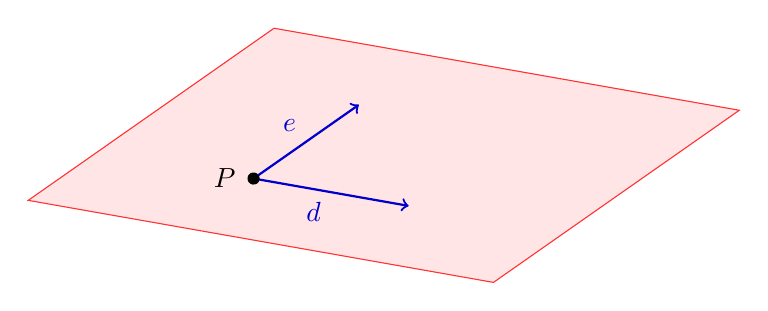
\begin{tikzpicture}[rotate=-10]
    % Note: I deliberately made the red a bit lighter and the blue a bit
    % darker, so that it will also look okay in black-and-white.
    \filldraw[draw=red!80,fill=red!10](-2,0,-5) -- (4,0,-5) -- (4,0,2) -- (-2,0,2) -- cycle;
    \draw[->,thick,blue!80!black](0,0,0) -- node[below left] {$\vect{d}$} (2,0,0);
    \draw[->,thick,blue!80!black](0,0,0) -- node[above left] {$\vect{e}$} (0,0,-3);
    \fill (0,0) circle [radius=2.2pt] node [left=3pt] {$P$};
  \end{tikzpicture}
\end{center}
The plane is infinite in each direction, although in the picture, we
have only shown a small part of it. If $\vect{p}$ is the position
vector of $P$ and $\vect{q}$ is the position vector of some other
point in the plane, we have
\begin{equation*}
  \vect{q} = \vect{p} + t\,\vect{d} + s\,\vect{e}
\end{equation*}
for some real numbers $t$ and $s$. This is called the \textbf{vector
  equation}%
\index{vector equation of a plane}\index{plane!vector equation} of the
plane.

\begin{definition}{Vector equation of a plane}{vector-equation-of-plane}
  Let $\vect{p}$ be a vector and let $\vect{d},\vect{e}$ be non-zero,
  non-parallel vectors. Then
  \begin{equation*}
    \vect{q} = \vect{p} + t\,\vect{d} + s\,\vect{e}
  \end{equation*}
  is the \textbf{vector equation}%
  \index{vector equation of a plane}\index{plane!vector equation} of a
  plane.
\end{definition}

The vector equation of a plane can also be written in
\textbf{component form}%
\index{vector equation of a plane!component form}%
\index{component form}\index{plane!component form}
\begin{equation*}
  \begin{mymatrix}{c} x_1 \\ x_2 \\ \vdots \\ x_n \end{mymatrix}
  = \begin{mymatrix}{c} p_1 \\ p_2 \\ \vdots \\ p_n \end{mymatrix}
  + t \begin{mymatrix}{r} d_1 \\ d_2 \\ \vdots \\ d_n \end{mymatrix},
  + s \begin{mymatrix}{r} e_1 \\ e_2 \\ \vdots \\ e_n \end{mymatrix}
\end{equation*}
and in \textbf{parametric form}
\begin{equation*}
  \begin{array}{c@{~}c@{~}c}
    x_1 &=& p_1 + t\,d_1 + s\,e_1, \\
    x_2 &=& p_2 + t\,d_2 + s\,e_2, \\
        &\vdots&             \\
    x_n &=& p_n + t\,d_n + s\,e_n.
  \end{array}
\end{equation*}
The latter set of equations are also called the \textbf{parametric
  equations}%
\index{parametric equations!of a plane}%
\index{plane!parametric equations} of the plane.

\begin{example}{Vector and parametric equations}{plane-from-three-points}
  Find vector and parametric equations for the plane through the
  points $P = \tup{1,2,0,0}$, $R = \tup{2,2,0,1}$, and $Q = \tup{0,1,1,0}$.
\end{example}

\begin{solution}
  We can use $P$ as the base point and $\longvect{PR}$ and
  $\longvect{PQ}$ as the direction vectors. We have
  \begin{equation*}
    \longvect{PR} =
    \begin{mymatrix}{c} 2\\2\\0\\1 \end{mymatrix}
    - \begin{mymatrix}{c} 1\\2\\0\\0 \end{mymatrix}
    = \begin{mymatrix}{c} 1\\0\\0\\1 \end{mymatrix}
    \quad\mbox{and}\quad
    \longvect{PQ} =
    \begin{mymatrix}{c} 0\\1\\1\\0 \end{mymatrix}
    - \begin{mymatrix}{c} 1\\2\\0\\0 \end{mymatrix}
    = \begin{mymatrix}{c} -1\\-1\\1\\0 \end{mymatrix}.
  \end{equation*}
  Therefore the vector equation is
  \begin{equation*}
    \begin{mymatrix}{c} x\\y\\z\\w \end{mymatrix}
    = \begin{mymatrix}{c} 1\\2\\0\\0 \end{mymatrix}
    + t\,\begin{mymatrix}{c} 1\\0\\0\\1 \end{mymatrix}
    + s\,\begin{mymatrix}{c} -1\\-1\\1\\0 \end{mymatrix}.
  \end{equation*}
  We can also write this as a system of parametric equations:
  \begin{equation*}
    \begin{array}{c@{~}c@{~}l}
      x &=& 1 + t - s, \\
      y &=& 2 - s, \\
      z &=& s, \\
      w &=& t.
    \end{array}
  \end{equation*}
\end{solution}

\begin{example}{Determine whether a point is on a plane}{point-on-plane-parametric}
  Determine whether the point $S=(4,4,-2,1)$ lies on the plane through
  the points $P = \tup{1,2,0,0}$, $R = \tup{2,2,0,1}$, and
  $Q = \tup{0,1,1,0}$.
\end{example}

\begin{solution}
  We already found the parametric equations for this plane in
  Example~\ref{exa:plane-from-three-points}. To determine whether the
  point $S=(4,4,-2,1)$ lies on this plane, we must substitute its
  coordinates into the parametric equations:
  \begin{equation*}
    \begin{array}{r@{~}c@{~}l}
      4 &=& 1 + t - s, \\
      4 &=& 2 - s, \\
      -2 &=& s, \\
      1 &=& t.
    \end{array}
  \end{equation*}
  This is a system of linear equations. We solve it to find that it
  has the unique solution $(t,s) = (1,-2)$. Therefore, the point $S$
  lies on the given plane, and more specifically, it is the point that
  corresponds to the parameters $t=1$ and $s=-2$.
\end{solution}

% ----------------------------------------------------------------------


Given a vector $\vect{n}$ in $\R^n$ and a point $P_0$, it is possible
to find a \textbf{unique} plane which contains $P_0$ and is
perpendicular to the given vector.

\begin{definition}{Normal vector}{normal-vector}
Let $\vect{n}$ be a nonzero vector in $\R^n$. Then $\vect{n}$ is called a \textbf{normal vector}\index{plane!normal vector} to a plane if and only if 
\[
\vect{n} \dotprod \vect{v} = 0
\]
for every vector $\vect{v}$ in the plane. 
\end{definition}

In other words, we say that $\vect{n}$ is orthogonal (perpendicular) to every vector in the plane. 

Consider now a plane with normal vector given by $\vect{n}$, and containing a point $P_0$. Notice that this plane is unique. If $P$ is an arbitrary point on this plane, then by definition the normal vector is orthogonal to the vector between $P_0$ and $P$. Letting $\longvect{0P}$ and $\longvect{0P_0}$ be the position vectors of points $P$ and $P_0$ respectively, it follows that 
\[
\vect{n} \dotprod (\longvect{0P} - \longvect{0P_0}) = 0 
\]
or
\[
\vect{n} \dotprod \longvect{P_0P} = 0 
\]

The first of these equations gives the \textbf{vector equation} of the plane. 

\begin{definition}{Vector equation of a plane}{vect-eqn-plane}
Let $\vect{n}$ be the normal vector for a plane which contains a point $P_0$. If $P$ is an arbitrary point on this plane, then the \textbf{vector equation}\index{plane!vector equation} of the plane is given by 
\[
\vect{n} \dotprod (\longvect{0P} - \longvect{0P_0}) = 0
\]
\end{definition}

Notice that this equation can be used to determine if a point $P$ is contained in a certain plane. 

\begin{example}{A point in a plane}{point-plane}
Let $\vect{n} = 
\begin{mymatrix}{r}
1 \\
2 \\
3 
\end{mymatrix}$ be the normal vector for a plane which contains the point $P_0 = \tup{2, 1, 4 }$. Determine if the point $P = \tup{5, 4, 1 }$ is contained in this plane. 
\end{example}

\begin{solution}
By Definition \ref{def:vect-eqn-plane}, $P$ is a point in the plane if it satisfies the equation
\[
\vect{n} \dotprod (\longvect{0P} - \longvect{0P_0}) = 0
\]

Given the above $\vect{n}$, $P_0$, and $P$, this equation becomes
\begin{eqnarray*}
\begin{mymatrix}{r}
1 \\
2 \\
3
\end{mymatrix}
\dotprod
\tup{
\begin{mymatrix}{r}
5 \\
4 \\
1
\end{mymatrix}
-
\begin{mymatrix}{r}
2 \\
1 \\
4
\end{mymatrix}
}
&=& 
\begin{mymatrix}{r}
1 \\
2 \\
3
\end{mymatrix}
\dotprod
\tup{
\begin{mymatrix}{r}
3 \\
3 \\
-3
\end{mymatrix}
} \\
&=& 
3 + 6 - 9 = 0
\end{eqnarray*}

Therefore $P = ( 5, 4, 1)$ is contained in the plane.

\end{solution}

Suppose $\vect{n} = \begin{mymatrix}{c}
a \\
b \\
c
\end{mymatrix}$, $P = \tup{x,y,z}$ and $P_0 = (x_0, y_0, z_0 )$.

Then 
\begin{eqnarray*}
\vect{n} \dotprod (\longvect{0P} - \longvect{0P_0}) &=& 0 \\
\begin{mymatrix}{c}
a \\
b \\
c
\end{mymatrix}
\dotprod
\tup{
\begin{mymatrix}{c}
x \\
y \\
z
\end{mymatrix}
-
\begin{mymatrix}{c}
x_0 \\
y_0 \\
z_0
\end{mymatrix}
} 
&=& 0 \\
\begin{mymatrix}{c}
a \\
b \\
c
\end{mymatrix}
\dotprod
\begin{mymatrix}{c}
x - x_0 \\
y - y_0 \\
z - z_0
\end{mymatrix}
&=& 0 
\\
a(x - x_0) + b (y - y_0) + c (z-z_0) &=& 0 
\end{eqnarray*}

We can also write this equation as 
\[
ax + by + cz = ax_0 + by_0 + cz_0
\]

Notice that since $P_0$ is given, $ax_0+by_0+cz_0$ is a known scalar, which we can call $d$. This equation becomes
\[
ax + by + cz = d
\]

\begin{definition}{Scalar equation of a plane}{scalar-eqn-plane}
Let $\vect{n} = \begin{mymatrix}{c}
a \\
b \\
c
\end{mymatrix} $
be the normal vector for a plane which contains the point $P_0 = (x_0, y_0, z_0)$.Then if $P=(x,y,z)$ is an arbitrary point on the plane, the \textbf{scalar equation}\index{plane!scalar equation} of the plane is given by
\[
ax + by + cz = d 
\]
where $ a,b,c,d \in \R$ and $d = ax_0 + by_0 + cz_0$.
\end{definition}

Consider the following equation.

\begin{example}{Finding the equation of a plane}{finding-eqn-plane}
Find an equation of the plane containing $P_0 = (3, -2, 5)$ and orthogonal to $\vect{n} = 
\begin{mymatrix}{r}
-2 \\
4 \\
1
\end{mymatrix}$. 
\end{example}

\begin{solution}
The above vector $\vect{n}$ is the normal vector for this plane.
Using Definition \ref{def:vect-eqn-plane}, we can determine the vector equation for this plane. 
\begin{eqnarray*}
\vect{n} \dotprod (\longvect{0P} - \longvect{0P_0}) &=& 0 \\
\begin{mymatrix}{r}
-2 \\
4 \\
1
\end{mymatrix} 
\dotprod 
\tup{\begin{mymatrix}{c}
x \\
y \\
z
\end{mymatrix}
-
\begin{mymatrix}{r}
3 \\
-2 \\
5
\end{mymatrix} } &=& 0 \\
\begin{mymatrix}{r}
-2 \\
4 \\
1
\end{mymatrix} 
\dotprod 
\begin{mymatrix}{c}
x - 3 \\
y + 2 \\
z - 5
\end{mymatrix}
&=& 0 
\end{eqnarray*} 

Using Definition \ref{def:scalar-eqn-plane}, we can determine the scalar equation of the plane. 
\[
-2x + 4y + 1z = -2(3) + 4(-2) + 1(5) = -9
\]

Hence, the vector equation of the plane is
\[
\begin{mymatrix}{r}
-2 \\
4 \\
1
\end{mymatrix} 
\dotprod 
\begin{mymatrix}{c}
x - 3 \\
y + 2 \\
z - 5
\end{mymatrix}
= 0 
\]
and the scalar equation is 
\[
-2x + 4y + 1z = -9
\]
\end{solution}

Suppose a point $P$ is not contained in a given plane. We are then interested in the shortest distance from that point $P$ to the given plane. Consider the following example. 

\begin{example}{Shortest distance from a point to a plane}{shortest-distance-plane}
Find the shortest distance from the point $P = (3,2,3)$ to the plane given by \\ $ 2x + y + 2z = 2$, and find the point $Q$ on the plane that is closest to $P$. 
\end{example}

\begin{solution}
Pick an arbitrary point $P_0$ on the plane. Then, it follows that
\[
\longvect{QP} = \func{proj}_{\vect{n}}\longvect{P_0P}
\]
and $\norm{\longvect{QP}}$ is the shortest distance from $P$ to the plane. Further, the vector $\longvect{0Q} = \longvect{0P} - \longvect{QP}$ gives the necessary point $Q$. 

From the above scalar equation, we have that $\vect{n} = 
\begin{mymatrix}{c}
2 \\
1 \\
2 
\end{mymatrix}$. Now, choose $P_0 = (1, 0, 0)$ so that $\vect{n} \dotprod \longvect{0P} = 2 = d$. 
Then, $\longvect{P_0P} = \begin{mymatrix}{c}
3 \\
2 \\
3
\end{mymatrix}
- 
\begin{mymatrix}{c}
1 \\
0 \\
0
\end{mymatrix}
=
\begin{mymatrix}{c}
2 \\
2 \\
3
\end{mymatrix}$. 

Next, compute $\longvect{QP} = \func{proj}_{\vect{n}}\longvect{P_0P}$. 
\begin{eqnarray*}
\longvect{QP} &=& \func{proj}_{\vect{n}}\longvect{P_0P} \\
&=& \tup{\frac{ \longvect{P_0P} \dotprod \vect{n}}{\norm{\vect{n}} ^2}}\vect{n} \\
&=& \frac{12}{9} \begin{mymatrix}{r}
2 \\
1 \\
2
\end{mymatrix} \\
&=& \frac{4}{3} \begin{mymatrix}{r}
2 \\
1 \\
2
\end{mymatrix} 
\end{eqnarray*}

Then, $\norm{\longvect{QP}} = 4$ so the shortest distance from $P$ to the plane is $4$. 

Next, to find the point $Q$ on the plane which is closest to $P$ we have
\begin{eqnarray*}
\longvect{0Q} &=& \longvect{0P} - \longvect{QP} \\
&=& \begin{mymatrix}{r}
3 \\
2 \\
3
\end{mymatrix} 
-
\frac{4}{3} \begin{mymatrix}{r}
2 \\
1 \\
2
\end{mymatrix} \\
&=& 
\frac{1}{3}
\begin{mymatrix}{r}
1 \\
2 \\
1
\end{mymatrix}
\end{eqnarray*}

Therefore, $Q = (\frac{1}{3}, \frac{2}{3}, \frac{1}{3} )$.  
\end{solution}
